\chapter{CleverMail}
\label{cha:clevermail}
In diesem Kapitel wird nun das Konzept von \emph{CleverMail} behandelt, welches die bestehende Anwendung \emph{CCMail} ablösen soll. Nachdem die Betrachtungen und Analysen von \emph{CCMail} abgeschlossen sind und einige Fehlentscheidungen ausgemacht wurden kann man sich jetzt dem Konzept für \emph{CleverMail} zuwenden. Im Gegensatz zu \emph{CCMail} wird aus der Sicht von \emph{CleverMail} das Gesamtsystem aus mehr Anwendungen bestehen, die in der Lage sein müssen E-Mail-Nachrichten zu versenden. Über die Zeit ist das GEsatmsystem \emph{clevercure} angewachsen und es wurden neue Anwendungen hinzugefügt, die Aufgrund der Architektur von \emph{CCMyail} nicht eingebunden werden konnten bzw. man sich dazu entschieden hat die Einbindung zu unterlassen.
\newline
\newline
Folgende Auflistung zeigt alle Anwendungen, die \emph{CleverMail} nutzen werden:
\begin{enumerate}
	\item\emph{CleverWeb}
	\newline
	Die Web-Anwendung für den webbasierten Zugriff auf das System
	\item\emph{CleverInterface}
	\newline
	Die Schnittstellen Anwendung für den Datenimport/-export
	\item\emph{CleverSupport (neu)}
	\newline
	Die Web-Anwendung für die Support Abteilung
	\item\emph{CleverDocument (neu)}
	\newline
	 Das Dokumentenmanagementsystem welches von allen Anwendungen genutzt wird
\end{enumerate}
Im Gegensatz zu \emph{CCMail} soll \emph{CleverMail} nicht als Konsolenanwendung implementiert werden sondern soll als Enterprise-Anwendung implementiert, welche als eigenständige Anwendung in einem JEE7-Applikationsserver betrieben wird.
\newpage
Mit dieser Art von Anwendung stehen \emph{CleverMail} eine Vielzahl von Features und Frameworks zur Verfügung wie z.B.: 
\begin{enumerate}
	\item JAX-RS 2.0\footnote{Java Api for RESTful Web Services 2.0. Java Api für REST Services}
	\item EJB 3.1\footnote{Enterprise Java Bean. Standard Komponenten für die Entwicklung in Java Enterprise Containern} 
	\item JPA 2.1\footnote{Java Persistence Api. Java Schnittstelle für Datenbankzugriffe} 
	\item JTA 1.2\footnote{Java Transaction Api. Java Schnittstelle für den Support von verteilten Transaktionen}
	\item JSF 2.2\footnote{Java Server Faces. Java Spezifikation für die Entwicklung von Webanwendungen basierend auf Java Server Pages (JSP)}
	\item uvm.
\end{enumerate}
Dies Features werden es erlauben die Anwendung \emph{CleverMail} so flexibel wie möglich zu gestalten, bringen aber auch ein erhöhtes Maß an Komplexität beim Design mit sich. Martin Fowler führt in seinem Buch \emph{Patterns of Enterprise Application Architecture}\cite[5-6]{patternsOfEnterprise} einige Beispiel für Enterprise-Anwendungen an um zu illustrieren dass jede dieser Anwendungen seine eigenen Probleme und Komplexität mit sich bringt und sich daher die Architektur einer Enterprise-Anwendung nicht einordnen und quantifizieren lässt. Daher ist beim Erstellen einer Architektur einer Enterprise-Anwendung der konkrete Nutzung zu berücksichtigen. Der Prozess der Konzeption einer Architektur ist ein kreativer Prozess wobei Konzepte, Best-Practise usw. nur als Unterstützung anzusehen sind und es keinen echten Leitfaden gibt an den man sich orientieren kann. Die Architektur wird stark von der konkreten Anwendung beeinflusst. Daher kann sich die Architektur je nach Anwendung stark unterschieden.
\newpage
\section{Systemaufbau}
Im Gegensatz zum Systemaufbau aus der Sicht von \emph{CCMail}, beschrieben in \ref{sec:ccmail-systemaufbau}, soll die Datenbank nicht mehr als Schnittstelle zwischen den Anwendungen und \emph{CleverMail} fungieren. Die Datenbank soll weiterhin ein zentraler Bestandteil von \emph{CleverMail} sein jedoch soll diese von den Anwendungen abstrahiert werden. Damit erreicht man dass die Anwendungen eine einheitliche Schnittstelle nutzen und nicht ihrerseits eigene Implementierungen warten müssen.
\begin{figure}[h]
\centering
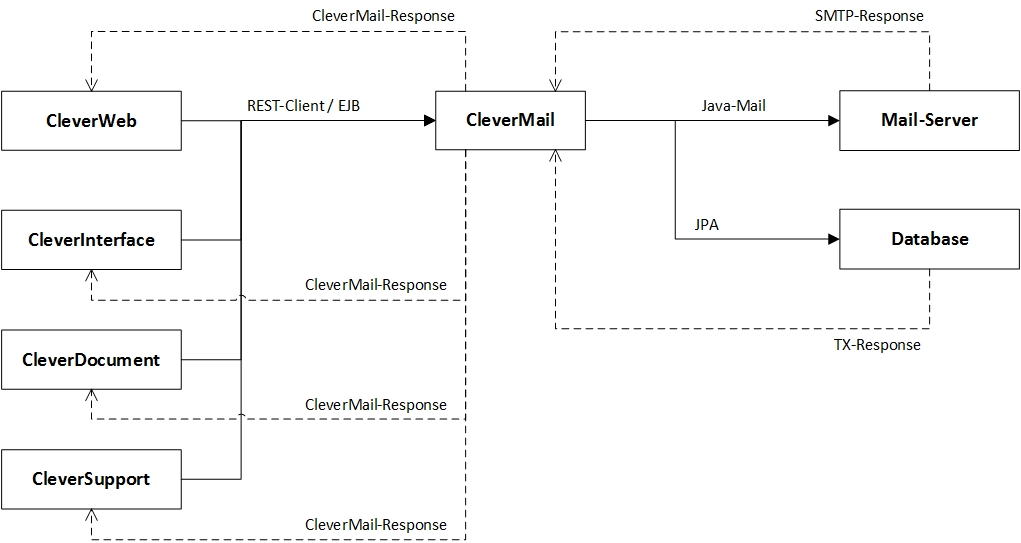
\includegraphics[scale=0.58]{clevermail_systemaufbau.jpg} %{CS0031}
\caption{Systemaufbau und Integration von \emph{CleverMail}}
\label{fig:clevermail-system-und-integration}
\end{figure}
\ \newline
Wie in der Abbildung \ref{fig:clevermail-system-und-integration} illustriert soll als zentrale Schnittstelle \emph{CleverMail} bzw. dessen implementierte Client-API fungieren wobei diese CLient-API sich wie folgt ausprägen könnte:
\begin{enumerate}
	\item\emph{REST-Client}
	\newline
	Eine REST-Schnittstelle zu einen REST-Webservice über den die zur verfügung gestellten Funktionalitäten genutzt werden können.
	\item\emph{EJB}
	\newline
	Ein EJB-Bean welches die zur Verfügung gestellten Funktionalitäten bereitstellt.
\end{enumerate}
\ \newline
\emph{CleverMail} seinerseits ist für die Persistenzschicht und das versenden der E-Mail-Nachrichten verantwortlich und trennt diese Aufgaben vollständig von den Anwendungen. So kann die Wartung nur an einer stelle erfolgen und muss nicht über alle Anwendungen hinweg erfolgen. In den Anwendungen würden nur noch Änderungen an den Schnittstellen Eingriffe erfordern.
\newpage
Dieser Ansatz würde das Problem der eigens implementierten Datenbankzugriffe \ref{sec:ccmail-systemaufbau} lösen. Ein Problem könnten hier etwaige technologische Unterschiede darstellen wie z.B.:
\begin{enumerate}
	\item REST nicht verfügbar
	\item EJB nicht verfügbar
	\item Falscher Source-Level
\end{enumerate}
\ \newline
Obwohl diese Probleme auftreten könnten kann zumindest gewährleistet werden, dass alle Anwendungen dieselbe Schnittstelle und dasselbe Domain-Model verwenden, selbst wenn eigene Implementierungen erforderlich sind. Diese Implementierungen würden eine Softwarekomponente von \emph{CleverMail} darstellen und währen auch Teil dieser Anwendung und dürfen nicht von den Anwendungen selbst bereitgestellt werden.
Diese technologischen Unterschiede könnten wie folgt gelöst werden.
\begin{enumerate}
	\item\emph{REST}
	\newline
	Integration von JAX-RS 2.0 
	\item\emph{EJB}
	\newline
	Integration eines EJB-Containers, zur Verfügung stellen eines Wrappers oder eine eigene Implementierung des spezifizierten Interfaces
\end{enumerate}
\subsection{REST-Client}
Eine REST-Client API, welche sich mit JAX-RS 2.0 einfach realisieren lässt, würde ein hohes Maß an Abstraktion bieten, nur eine geringe Kopplung aufweisen und wenig Abhängigkeiten in der Anwendung erfordern. Dies steht aber gegenüber dass REST-Services zustandslos sind und sich daher implizit nicht in Datebank 
Transaktionen einbinden lassen. Dies könnte aber erforderlich sein wenn eine E-Mail nur dann angelegt und versendet werden darf wenn die Transaktion erfolgreich abgeschlossen wurde (z.B.: Anlegen einer Bestellung). Würde über den REST-Service eine E-Mail Nachricht angelegt werden. Für einen REST-Service startet eine Transaktion mit dessen Aufruf und endet mit dem Übermitteln der Response oder wenn die Aktion abgeschlossen wurde (asynchron).
\newpage
Für diese Problem gibt es eine Lösung in Form eines Konzeptes mit der Bezeichnung Try-Confirm-Cancel (TCC).
\begin{figure}[h]
\centering
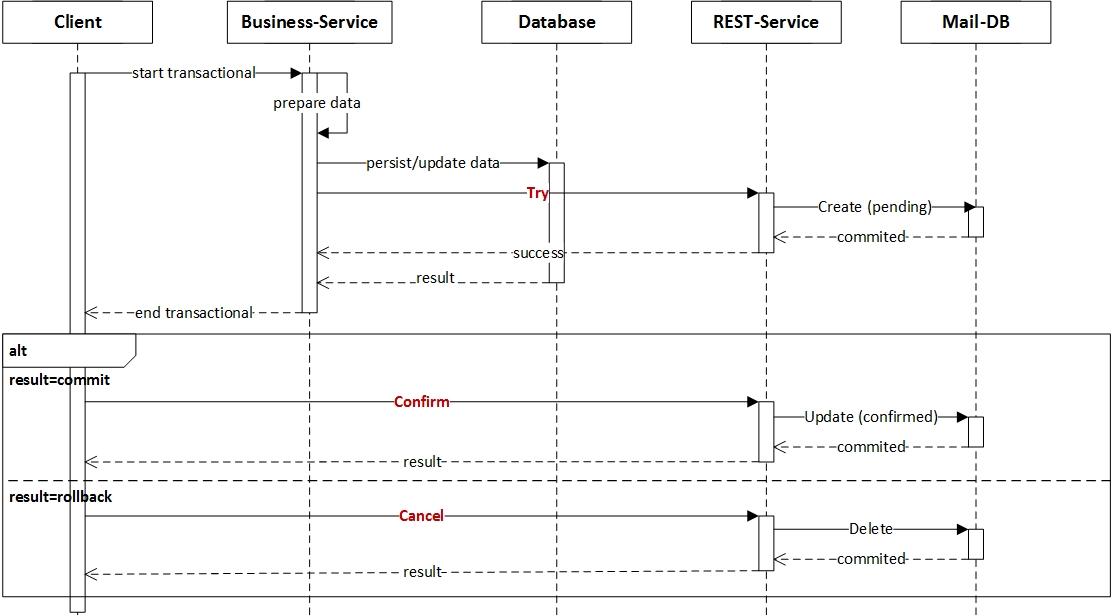
\includegraphics[scale=0.5]{try_confirm_cancel.jpg} %{CS0031}
\caption{Beispiel einer Transaktion mit TCC}
\label{fig:clevermail-rest-tcc}
\end{figure}
\ \newline
Mit diesem Konzept müsste der REST-Service den Zustand persistent halten aber als \emph{unconfirmed} markieren, damit dieser in keiner Verarbeitungslogik miteinbezogen wird. Nachdem erfolgreichen Abschluss der Transaktion auf der Client-Seite muss dieser durch den REST-Service persistent gehaltenen Zustand bestätigen und im Falle eines Fehlers abbrechen. Dies würde zwei Aufrufe zu REST-Services verursachen. Ebenfalls sollte die Transaktion über einen Transaktionskoordinator auf der REST-Seite kontrolliert werden, was wieder einen Mehraufwand bedeutet. Dieser Transaktionskoordinator ist dafür verantwortlich die REST-Services, die Teil einer logischen Transaktionen sind,  zu managen. Mit \emph{TCC} besteht auch die Gefahr das eine Heuristic-Exception auftritt. Beim Auftreten einer solchen Exception würden inkonsistente Datenbestände auf der Datenbank entstehen, da es sein könnte das nicht alle REST-Services ein Rollback durchgeführt haben.
\newline
\newline
Diese Probleme bedeuten aber nicht dass REST-Services nicht in Frage kommen. Lediglich für transaktionale Operationen scheinen sie ungeeignet bzw. der Aufwand der betrieben werden muss zu hoch. Ein weiteres Problem könnte die Erreichbarkeit dieser REST-Services sein. Sollte dieser einmal ausfallen oder im Falle eines Deployments nicht erreichbar sein so müsste man eine Rückversicherung haben und die zu erstellenden E-Nachrichten anderweitig zwischenspeichern wie z.B.: in Form einer Textdatei, welche die Daten als JSON enthält.
\newline
\newline
Diese Onlinepublikation \cite{atomikosTcc} beschreibt den Prozess von \emph{TCC} mit mehreren involvierten REST-Services sehr gut und detailliert.
\subsection{EJB}
Sollte eine Anwendung über EJB mit \emph{CleverMail} kommunizieren so würde hierbei eine starke Kopplung und starke Abhängigkeiten entstehen, da hier mehr Ressourcen benötigt werden. Ebenso könnte im Gegensatz zu einem REST-Client keine eigene Datenbank genutzt werden, da hier ein Zweiphasen-Commit erfolgen müsste. Natürlich würde diese Möglichkeit bestehen aber auch hier wäre man der Gefahr von Heursitc-Exceptions ausgesetzt.
\begin{figure}[h]
\centering
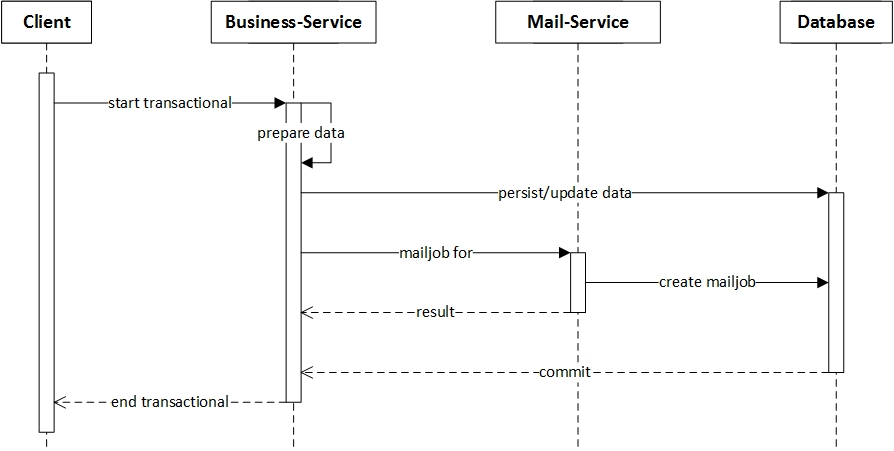
\includegraphics[scale=0.5]{clevermail-ejb-transaktion.jpg} %{CS0031}
\caption{Beispiel einer EJB (JTA) Datenbanktransaktion}
\label{fig:clevermail-rest-tcc}
\end{figure}
\ \newline
In diesem Fall würde das Anlegen einer E-Mail in derselben Transaktione erfolgen und würde daher auch im Falle eines Roolbacks entfernt werden. Dies ist sicher die angenehmste Art und Weise um E-Mails anzulegen, da hier keine besonderen Mechanismen implementiert werden müssten um die Datenkonsistenz zu gewährleisten. Hierbei währen die E-Mail-Nachrichten auch Teil einer wohl definierten Transaktion.
\newline
\newline
Wie hier \ref{cha:clevermail} angemerkt können technologische Probleme auftreten wenn z.B.: eine Anwendung kein \emph{EJB} und/oder \emph{JPA} unterstützt. Hierbei müsste man eine eigene Implementierung erstellen, die zumindest Teil von \emph{CleverMail} sein sollte.
\newline
\newline
Dieser transaktionale Ansatz unterschiedet sich nicht von dem in \emph{CCMail} bereits implementierten jedoch sollen hier die von \emph{CleverMail} zur Verfügung gestellten implementierten Ressourcen verwendet werden. Diese Ressourcen sollten auch im Backend der REST-Services von \emph{CleverMail} angewandt werden, da auch hier die Persistenz der E-Mails gewährleistet werden muss. 
\newpage
\chapter{Prozesse}
\label{cha:clevermail-prozesse}
Diese Kapitel behandelt die Prozessspezifikationen von \emph{CleverMail}. Hierbei wird das Augenmerk auf den Mailversand gelegt. Grundlegend wird sich der E-Mail-Versand dadurch unterschieden, dass hier mehrere Ebenen involviert sind, bevor eine E-Mail-Nachricht bereit zum Versand ist. Vom grundlegenden Konzept wird sich gegenüber \emph{CCMail} nicht viel ändern. Es soll immer noch E-Mail-Typen geben, die aber jetzt nicht nur intern konfigurierbar sein sollen sondern ebenfalls durch die Kunden selbst konfiguriert und gesteuert werden können. Hierbei sollen folgende Konfigurationsmöglichkeiten zur Verfügung stehen.
\begin{enumerate}
	\item Definition von Schedules
	\item Definition eigener E-Mail-Vorlagen
	\item Konfiguration der Steuerbarkeit von E-Mail-Typen durch Lieferanten (darf aktivieren/de-aktivieren)
	\item Definition eines Haftungsausschluss 
	\item Definition von Standard Datei Anhängen
	\item Steuerbarkeit von E-Mail-Typen für spezifischen Lieferanten
	\item Konzernübergreifende Konfiguration
	\item Definition eigener E-Mail-Typen
	\item Konfiguration der Historie der E-Mail-Nachrichten
\end{enumerate}
\ \newline
Zur Zeit stehen diese Features, wenn vorhanden, nur intern zur Verfügung. Die Kunden haben lediglich die Möglichkeit einzelne E-Mail-Typen zu aktivieren oder zu de-aktivieren. Diese E-Mail-Typen können aber mehrere E-Mail-Nachrichten beinhalten. Das Grundlegende Ziel ist das die Kunden mehr Kontrolle und Konfigurationsmöglichkeiten über die zur Verfügung gestellten E-Mail-Typen erhalten. Es wird hier aber auch solche E-Mail-Typen geben, bei denen diese Konfigurationsmöglichkeiten eingeschränkt werden. Nichts desto trotz soll der Kunde in der Lage sein, den E-Mail-Verkehr seiner E-Mail-Nachrichten besser zu steuern.
\newpage
\section{E-Mail-Versand}
\begin{figure}[h]
\centering
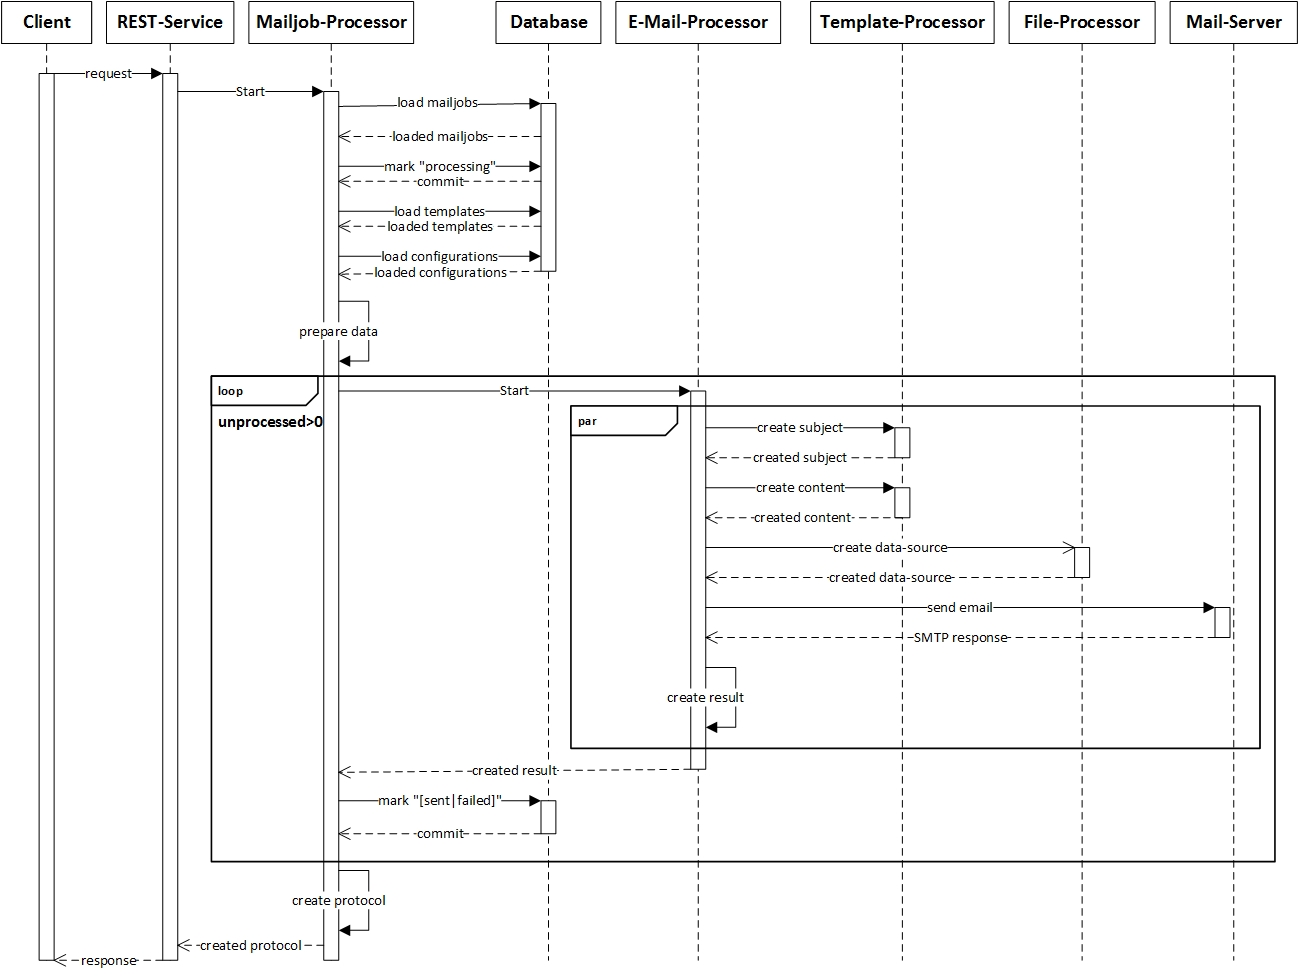
\includegraphics[angle=90, scale=0.6]{clevermail-email-versand.jpg} %{CS0031}
\caption{Prozess des E-Mail-Versands}
\label{fig:clevermail-email-versand}
\end{figure}
\ \newpage
Die Abbildung \ref{fig:clevermail-email-versand} soll den Prozess des E-Mail-Versands veranschaulichen und illustriert die involvierten Komponenten, die involviert sind um eine E-Mail-Nachricht zu erstellen. In diesem Beispiel wird der Prozess über einen REST-Service gestartet, der in diesem Fall den Prozess synchron abarbeitet und anschließend eine Response in Form eines erstellten Reports zurückliefert. Der REST-Service ist hierbei als optional anzusehen, da dieser Prozess auch anderweitig ausgelöst werden könnte. Nachdem sich dieser Prozess nicht in einer Transaktion eines Client befinden muss würde sich hier eine REST-Schnittstelle anbieten.
\newline
\newline
Folgende sei der Prozess in grobe Schritte unterteilt angeführt und beschrieben.
\subsection{Daten Aufbereitung}
Nachdem der Prozess gestartet wurde sollen die zu verarbeitenden E-Mail-Nachrichten aus der Datenbank ausgelesen und als \emph{Processing} markiert. Im Punkt \ref{sec:ccmail-gesamtprozess} wurde angemerkt, dass das Problem bestand ,dass die in Verarbeitung stehenden \emph{MailJob} Entitäten nicht als solche markiert wurden und daher eine parallele Verarbeitung durch mehrere Prozesse nicht möglich war. Dieses Problem besteht in diesem Fall nun nicht mehr. Nachdem die \emph{MailJob} geladen wurden sollen die zugrunde liegenden E-Mail-Vorlagen geladen werden. Hierbei würde sich ein Cache-Mechanismus auszahlen, da die E-Mail-Vorlagen Versionen definieren und sich innerhalb einer Version nicht ändern dürfen. Anschließend sollen die kundenspezifischen Konfigurationen geladen werden. Aus diesen Daten sollen Modelle erstellt werden, die in weitere Folge dazu verwendet werden sollen die E-Mail-Nachrichten zu erstellen.
\subsection{Erstellen der E-Mail-Nachrichten}
Aus den Modellen sollen die E-Mail-Nachrichten erstellt werden. Hierbei wird dieser Prozess in drei Schritte unterteilt.
\begin{enumerate}
	\item\emph{Erstellen des Betreff}
	\newline
	Der Betreff wird aus einer E-Mail-Vorlage erstellt und mit Daten befüllt sollten in der Voralge Parameter definiert worden sein
	\item\emph{Erstellen der Nachricht}
	\newline
	Die Nachricht wird aus einer E-Mail-Vorlage erstellt und mit Daten befüllt sollten in der Voralge Parameter definiert worden sein
	\item\emph{Erstellen der DataSoruces}
	\newline
	Sollten Datei Anhänge definiert worden sein, so werden diese in Form von einer oder mehrerer DataSoruce Instanzen in die E-Mail-Nachricht angefügt.
\end{enumerate}
\ \newline
Die Verarbeitung der E-Mail-Vorlagen soll in einer Komponente mit dem Name \emph{Template-Processor} erfolgen. Nachdem die Werte der verwendeten Vorlagenparameter beim Erstellen eines \emph{MailJob} in der Datenbank gespeichert wurden können diese hier angewandt werden.
\newline
\newline
Die Verarbeitung der Datei Anhänge soll in einer Komponente mit dem Namen \emph{File-Processor} erfolgen, die die verlinkten Datei Anhänge in Form von \emph{DataSource} Instanzen der E-Mail-Nachricht zur Verfügung stellt. Beim Versand würde die E-Mail-Nachricht den Datei Anhang über diese \emph{DataSource} Instanz laden. Hierbei sollen die Dateien in Form von Links aus dem Dokumentenmanagementsystem \emph{CleverDocument} geladen werden. Es soll keine Dateien in Form von Base64-Zeichenketten in der Datenbank mehr geben. Es könnten hierbei verschiedene \emph{DataSource} Implementierungen zur Verfügung gestellt werden, die die Dateien aus verschiedenen Quellen über die verschiedensten Protokolle laden können (z.B.: REST, SOAP, HTTP, usw.).
\subsection{E-Mail versenden}
Der E-Mail-Versand sowie das Erstellen der E-Mail-Nachricht sollte hierbei asynchron erfolgen, da eine sequenzielle Verarbeitung die Performance negativ beeinflussen würde. Nach dem erfolgreichen oder fehlgeschlagenen Versand einer E-Mail-Nachricht soll dieser Status in Form eines Resultates zurückgeliefert werden. Hierbei ist vor allem die SMTP-Response wichtig, die auf jeden Fall gespeichert werden soll damit der Kunde nachvollziehen kann wie der E-Mail-Versand seiner E-Mail abgearbeitet wurde und warum die E-Mail nicht zugestellt werden konnte. Ein fehlgeschlagener Versand könnte folgende Ursachen haben:
\begin{enumerate}
	\item Datei kann nicht geladen werden (nicht vorhanden, Timeout,...)
	\item Mail-Server des Empfängers nicht erreichbar
	\item E-Mail-Server nimmt Nachricht nicht an
	\item uvm.
\end{enumerate}
\ \newline
Es kann unzählige Ursachen haben warum eine E-Mail-Nachricht nicht zugestellt werden kann. Die trifft vor allem auf den E-Mail-Servers des Empfängers zu, auf dessen Konfiguration kein Einfluss genommen werden kann.
\newpage
\section{E-Mail-Vorlagenparameter}
Ein weiterer wichtiger Aspekt stellen die Vorlagenparameter und deren Verwaltung dar. Die Bereitstellung von Vorlagenparametern soll den AnwenderInnen die Möglichkeit bieten auf kontextabhängige Daten in einer E-Mail-Vorlage zugreifen zu können. Dadurch soll die Flexibilität erhöht werden und die AnwenderInnen sollen mehr Freiheiten beim Erstellen einer E-Mail-Vorlage bekommen. Diese Parameter müssen hierbei von den EntwicklerInnen innerhalb eines Kontextes zur Verfügung gestellt werden, wobei hier auch ein Entwicklungsaufwand besteht. Diese Parameter müssen beim Verarbeiten einer E-Mail-Vorlage aus dem aktuellen Kontext ausgelesen werden. Dabei können die Daten aus verschiedenen Objekten oder sogar Objektgraphen kommen. Dies bedeutet das diese Parameter über eine spezielle Implementierung ausgelesen werden müssen, die auch zukünftig gewartet werden muss. Ebenso werden diese Parameter in verschiedenen Softwarekomponenten verwendet die sich in verschiedenen Laufzeitumgebungen genutzt werden können. Daher wird es erforderlich sein diese Parameter in einem spezifizierten Model oder über definierte Zuordnungen von einem Model in ein anderes Model zu überführen.
\begin{figure}[h]
\centering
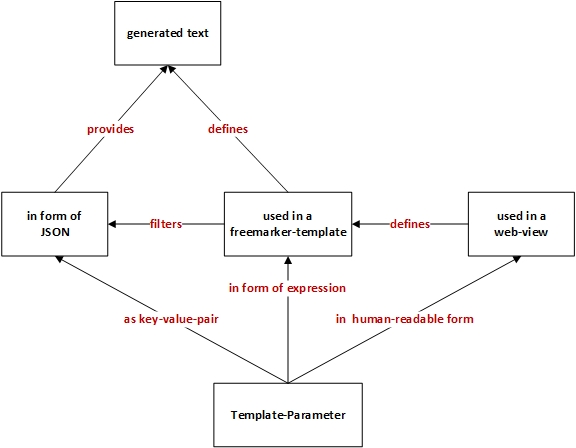
\includegraphics[scale=0.6]{clevermail_template_parameter.jpg}
\caption{Verwendung Vorlagenparameter}
\label{fig:clevermail-template-parameter}
\end{figure}
\ \newline
Wie in der Abbildung \ref{fig:clevermail-template-parameter} illustriert werden die Vorlagenparameter in mehreren Kontexten verwendet. Dadurch stellt sich die Frage wie diese Parameter adressiert werden. Man könnte eine Zuordnung in jedem Verwendungskontext erstellen, also jeder Kontext bekommt sein eigenes Model. Dadurch würde man sich zwar lose and die Vorlagenparameter koppeln jedoch erhält man auch eine Model Klasse je Kontext, die gewartet werden muss. 
\subsection{Webseite}
\label{sec:template-parameter-web-view}
Da diese Parameter in E-Mail-Vorlagen verwendet werden wird es auch eine Webseite geben, über die die AnwenderInnen diese Parameter in Ihren E-Mail-Vorlagen verwenden können. Diese müssen natürlich für die AnwenderInnen einen Name bekommen, der natürlich auch in mehreren Sprachen zur Verfügung stehen muss. Dadurch werden diese Parameter auf einen Schlüssel zugeordnet werden müssen, der wiederum auf einen lokalisierten Spracheintrag zugeordnet ist. Die Zuweisung auf diesen Schlüssel ist erforderlich aber benötigt man hier auch nochmals eine Zuordnung auf den Vorlagenparameter?
\subsection{Freemarker}
\label{sec:template-parameter-freemarker}
Ein weiterer Aspekt ist auch die direkte Verwendung der Parameter in der Vorlage selbst. Als Implementierung einer \emph{Template-Enging} soll für die Erstellung der Nachrichten aus den Vorlagen \emph{Freemarker}\footnote{\label{fn:freemarker}Frei verfügbare Template-Engine in Java für die Erstellung von dynamischen Textdateien} verwendet werden. Dieses Framework ist ein sehr beliebtes und gut gewartetes Framwork, welsche alle benötigten Kontrollstrukturen sowie \emph{Freemarker-Expressions} zur Verfügung stellt. Diese \emph{Freemarker-Expressions} ähneln sehr den Java-EL-Expressions\footnote{Java-Expression-Language ist eine Java Spezifikation für Expressions}. 
Die Vorlagenparameter werden in den \emph{Freemarker-Expressions} verwendet, die es ermögliche eine flache Adressierung sowie auch eine Adressierung über Objektgraphen zu definieren. Dadurch stellt sich auch hier die Frage ob diese Expressions wieder über eine Zuordnung zu den Parametern erstellt werden sollen oder ob die Parameter selbst verwendet werden?
\subsection{JSON}
\label{sec:template-parameter-json}
Wenn eine E-Mail in Form eines \emph{MailJob} erstellt wird müssen zum jeweiligen Erstellungszeitpunkt alle Parameterwerte ausgelesen und mit dem \emph{MailJob} persistent gehalten werden. Nachdem die Anzahl der Parameter dynamisch ist und diese Daten lediglich in der Vorlagenverarbeitung verwendet werden ist es hier nicht erforderlich eine eigene Datenstruktur auf der Datenbank zu definieren. Dadurch würde sich hier \emph{JSON} anbieten um diese Daten in die Datenbank zu serialisieren. Nachdem \emph{JSON} eine Objektbeschreibung darstellt und auch über ein \emph{JSON-Schema} spezifiziert kann sollte man überlegen ob man nicht das \emph{JSON} als Spezifikation für die Vorlagenparameter heranzieht. Diese Spezifikation kann in allen involvierten Komponenten verwendet werden. 
\newpage
\chapter{Datenbank}
Eine Anforderung an \emph{CleverMal} ist die Persistenz der versendeten E-Mail-Nachrichten damit diese einerseits nachvollziehbar sind und andererseits den AnwenderInnen die Möglichkeit geboten wird bereits versendete E-Mail-Nachrichten erneut zu versenden. Daher wird ein Speichermedium benötigt um diese E-Mail-Nachrichten persistent zu halten. Nachdem hier auch relationale Beziehungen vorhanden sein werden bittet sich natürlich eine Datenbank an. Neben den E-Mail-Nachrichten selbst müssen auch die E-Mail-Vorlagen sowie Konfigurationsdaten persistent gehalten werden. Die AnwenderInnen, die EntwicklerInnen und sowie auch die Support MitarbeiterInnen müssen in der Lage sein den E-Mail-Versand zu konfigurieren.
\newline
\newline
Die Datenbanktabellen lassen mittels \emph{JPA} in Java sehr gut ansprechen und man wird nur geringfügig sich direkt auf der Datenbankebene bewegen müssen. Im Gegensatz zu dem beschrieben Datenbankschemata in \ref{sec:ccmail-datanbank} soll hierbei keineswegs auf die referenzielle Integrität verzichtet werden. Man kann davon ausgehen das die Datenmenge und die Zugriffe auf diese Daten so schnell kein Niveau erreichen werden, die einen Verzicht auf die referenzielle Integrität rechtfertigen würde. Auch soll dieses Datenbankschemata ohne Referenzen auf bereits bestehende Tabellen auskommen. Es werden Beziehungen von Nöten sein, die man über n-m Tabellen abgebildet werden können. Damit referenzieren sich die Datenbankschemata in das Datenbankschemata von \emph{CleverMail} und nicht umgekehrt. Dadurch wird soll gewährleistet werden dass \emph{CleverMail} auch in anderen Anwendungen im clevercure Ökosystem eingebunden werden kann. Als Beispiel sei hier \emph{CleverSupport} angeführt, dass seinerseits auch ein eigenes Datenbankschemata hat, welches nicht mit dem Datenbankschemata der Hauptanwendung verbunden ist.
\newpage
\subsection{Datenbankschemata CleverMail}
\begin{figure}[h]
\centering
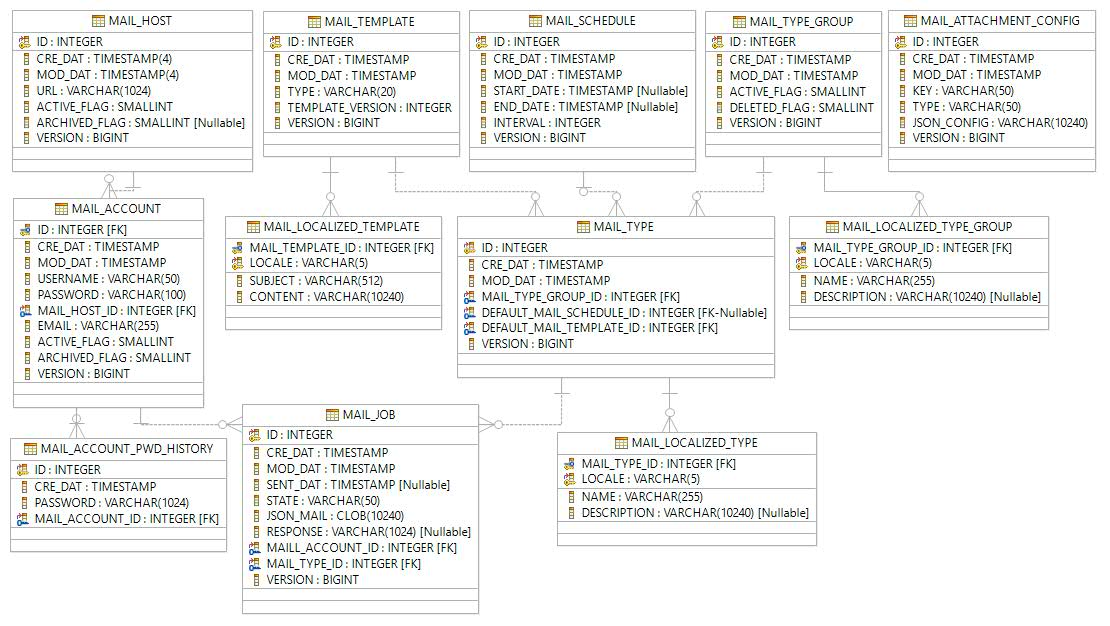
\includegraphics[angle=90, scale=0.4]{clevermail_db_schema.jpg}
\caption{Datenbankschema CleverMail}
\label{fig:clevermail-db-schema}
\end{figure}